\documentclass[aspectratio=169,11pt]{beamer}
\usepackage[utf8]{inputenc}
\usepackage[T1]{fontenc}
\usepackage{lmodern}
\usepackage{graphicx}
\usepackage{booktabs}
\usepackage{amsmath}
\usepackage{xcolor}

% --- tampilan bersih, satu warna aksen ---
\definecolor{tinta}{RGB}{22,28,38}
\definecolor{aksen}{RGB}{16,74,132}
\definecolor{merah}{RGB}{176,48,48}
\definecolor{hijau}{RGB}{28,120,72}
\definecolor{abu}{RGB}{120,128,138}

\usetheme{default}
\setbeamertemplate{navigation symbols}{}
\setbeamercolor{frametitle}{fg=aksen}
\setbeamercolor{title}{fg=aksen}
\setbeamercolor{structure}{fg=aksen}
\setbeamercolor{normal text}{fg=tinta}
\setbeamerfont{frametitle}{series=\bfseries}
\setbeamertemplate{itemize items}[circle]
\setbeamertemplate{frametitle}{%
  \vskip0.55em\hspace{0.3em}\usebeamerfont{frametitle}\insertframetitle\par
  \vskip-0.15em\hspace{0.3em}{\color{aksen}\rule{0.4\linewidth}{1.1pt}}}
\graphicspath{{figures/}}

\newcommand{\naik}[1]{{\color{hijau}\textbf{#1}}}
\newcommand{\turun}[1]{{\color{merah}\textbf{#1}}}
\newcommand{\key}[1]{{\color{aksen}\textbf{#1}}}

\title{\textbf{Analisis TFP}}
\subtitle{Produktivitas total faktor dengan \emph{returns to scale} tak direstriksi (non-CRS / DRS)}
\date{21 Juli 2026}

\begin{document}

\begin{frame}[plain]\titlepage\end{frame}

% ======================= BAGIAN 1: KONTEKS & METODE =======================
\begin{frame}{Intinya dulu}
  \Large
  \begin{itemize}
    \setlength\itemsep{0.8em}
    \item Angka TFP lama dikunci pakai asumsi \key{CRS}. Data menolak asumsi itu, jadi kami buka.
    \item TFP nasional yang tadinya seolah \turun{$-$0,27\%/th} ternyata \naik{$+$0,81\%/th}.
    \item Modal tetap penggerak utama: \key{64\%} dari pertumbuhan.
  \end{itemize}
  \vfill
  {\color{abu}\normalsize Slide berikut menjelaskan modelnya, kenapa CRS ditolak, dan seberapa besar taruhannya.}
\end{frame}

\begin{frame}{Apa yang kita ukur}
  Pertumbuhan output punya tiga sumber:
  \vspace{0.4em}
  \begin{enumerate}
    \setlength\itemsep{0.5em}
    \item \key{Tambah modal} (mesin, gedung, infrastruktur)
    \item \key{Tambah tenaga kerja}
    \item \key{Makin efisien memakainya} $\;\Rightarrow\;$ inilah \key{TFP}
  \end{enumerate}
  \vspace{0.8em}
  TFP tak bisa dipotret langsung. Kita hitung sebagai \textbf{sisa} setelah kontribusi
  modal dan tenaga kerja dikeluarkan:
  \[
    \underbrace{\log \mathrm{TFP}_{it}}_{\text{sisa}}
    \;=\; \log Y_{it} \;-\; \beta_1 \log K_{it} \;-\; \beta_2 \log L_{it}
  \]
  {\color{abu}\small $Y$ = PDRB riil, $K$ = PMTB, $L$ = tenaga kerja. Kunci semuanya ada di $\beta_1,\beta_2$.}
\end{frame}

\begin{frame}{Tiga skala hasil: CRS, DRS, IRS}
  \emph{Returns to scale}: kalau \textbf{semua} input digandakan, output naik berapa kali lipat?
  Jawabannya = jumlah elastisitas $\beta_1+\beta_2$.
  \vspace{0.5em}
  \begin{itemize}
    \setlength\itemsep{0.5em}
    \item \key{CRS} ($\beta_1{+}\beta_2{=}1$): output pas 2$\times$. Patokan \emph{growth accounting}.
    \item \key{DRS} ($<1$): output $<2\times$. Tambah input proporsional $\Rightarrow$ hasilnya menyusut.
    \item \key{IRS} ($>1$): output $>2\times$. Aglomerasi/klaster; skala hasil 1,01--1,10.
  \end{itemize}
  \vspace{0.5em}
  \textbf{Studi kasus.} ``Keajaiban Asia Timur'' (Young 1995; Krugman 1994): tumbuh pesat dari
  \key{akumulasi} input, TFP tipis $\Rightarrow$ \turun{melandai} saat akumulasi mentok ---
  ``\emph{perspiration}, bukan \emph{inspiration}'', persis pola Uni Soviet.
  \vspace{0.3em}
  {\color{abu}\small Data kita: $\beta_1{+}\beta_2=\key{0{,}591}$ (DRS terukur). IRS \textbf{tidak} ditemukan.}
\end{frame}

\begin{frame}{Kenapa investasi yang sama berbuah beda}
  Tambah modal = gerak \emph{sepanjang} fungsi produksi (bobot $\beta_1$). Karena $\beta_1<1$,
  \key{tiap unit modal tambahan berbuah makin kecil} --- \emph{diminishing returns}, berlaku bahkan di CRS.
  \vspace{0.4em}
  \begin{itemize}
    \setlength\itemsep{0.45em}
    \item Rupiah investasi sama, hasil beda tergantung: \key{ke mana} modal mengalir (sektor
          produktif vs rente SDA), \key{pasangannya} (TK terampil, teknologi), \key{utilisasi} kapasitas.
    \item Semua itu masuk \key{TFP} --- ``pengganda efisiensi'' yang menggeser \emph{seluruh} fungsi ke atas.
  \end{itemize}
  \vspace{0.4em}
  \textbf{Contoh dari data:} sisa \naik{Jawa $+$1,24} vs \turun{Kalimantan $-$0,11} poin. Kalimantan:
  input tumbuh lebih cepat dari output (investasi ekstraktif padat modal), bukan sekadar ``tak efisien''.
  \vspace{0.2em}
  {\color{abu}\small TK serupa: jumlah pekerja vs mutunya --- kenaikan mutu jatuh ke TFP, bukan ke kontribusi TK.}
\end{frame}

\begin{frame}{Model estimasinya}
  \[
    \log Y_{it} = \alpha + \beta_1 \log K_{it} + \beta_2 \log L_{it}
    + \underbrace{u_i}_{\text{efek provinsi}} + \underbrace{\lambda_t}_{\text{efek tahun}} + \varepsilon_{it}
  \]
  \vspace{0.2em}
  \begin{itemize}
    \setlength\itemsep{0.55em}
    \item \key{Panel 34 provinsi $\times$ 2017--2024} ($N=272$). Cobb--Douglas.
    \item \key{Two-way fixed effects} (efek tetap 2 arah): $u_i$ menyerap karakter
          tetap tiap provinsi, $\lambda_t$ menyerap guncangan makro bersama.
    \item \key{Driscoll--Kraay standard errors}: galat baku yang tahan korelasi
          antar-provinsi (uji Pesaran CD menolak independensi, $z=4{,}24$).
  \end{itemize}
  \vspace{0.5em}
  Hasil: $\;\beta_1 = \key{0{,}400}\ (\text{SE }0{,}053),\quad \beta_2 = \key{0{,}191}\ (\text{SE }0{,}068)$.
\end{frame}

\begin{frame}{FE tidak membuang keunikan wilayah}
  Kekhawatiran wajar: ``kalau kontrol provinsi \& tahun, bukankah keunikan tiap
  daerah malah hilang?'' \key{Tidak.}
  \vspace{0.8em}
  \begin{itemize}
    \setlength\itemsep{0.6em}
    \item Efek provinsi $u_i$ \key{tidak} jadi variabel penjelas. Dia masuk ke
          \textbf{residual}, artinya jadi \key{bagian dari TFP itu sendiri}.
    \item $u_i$ = level produktivitas khas tiap provinsi $\Rightarrow$ dipakai untuk \key{peringkat provinsi}.
    \item $\lambda_t$ = pergerakan produktivitas bersama tiap tahun $\Rightarrow$ dipakai untuk \key{indeks TFP nasional}.
  \end{itemize}
  \vspace{0.7em}
  {\color{abu} Yang dibersihkan FE cuma bias endogenitas input, bukan produktivitasnya.}
\end{frame}

\begin{frame}{Kenapa CRS ditolak, dan kenapa itu penting}
  \begin{columns}[T]
    \begin{column}{0.55\textwidth}
      \emph{Returns to scale} = seberapa besar output naik kalau semua input
      digandakan. \textbf{\color{aksen}CRS}: pas 2$\times$ ($\beta_1{+}\beta_2{=}1$).
      \textbf{\color{aksen}DRS}: kurang dari 2$\times$ ($<1$).
      \vspace{0.6em}

      Data bilang jumlahnya \key{0,591} (uji Wald menolak CRS, $p<0{,}001$) --- jadi DRS.
      \vspace{0.9em}

      \textbf{Bahayanya memaksa CRS:} sisa pertumbuhan input $(1-0{,}591)$ tak
      punya tempat, lalu \textbf{nyelinap ke residual dan dicap TFP}. TFP jadi
      terlihat kecil / negatif secara artifisial.
    \end{column}
    \begin{column}{0.43\textwidth}
      \centering
      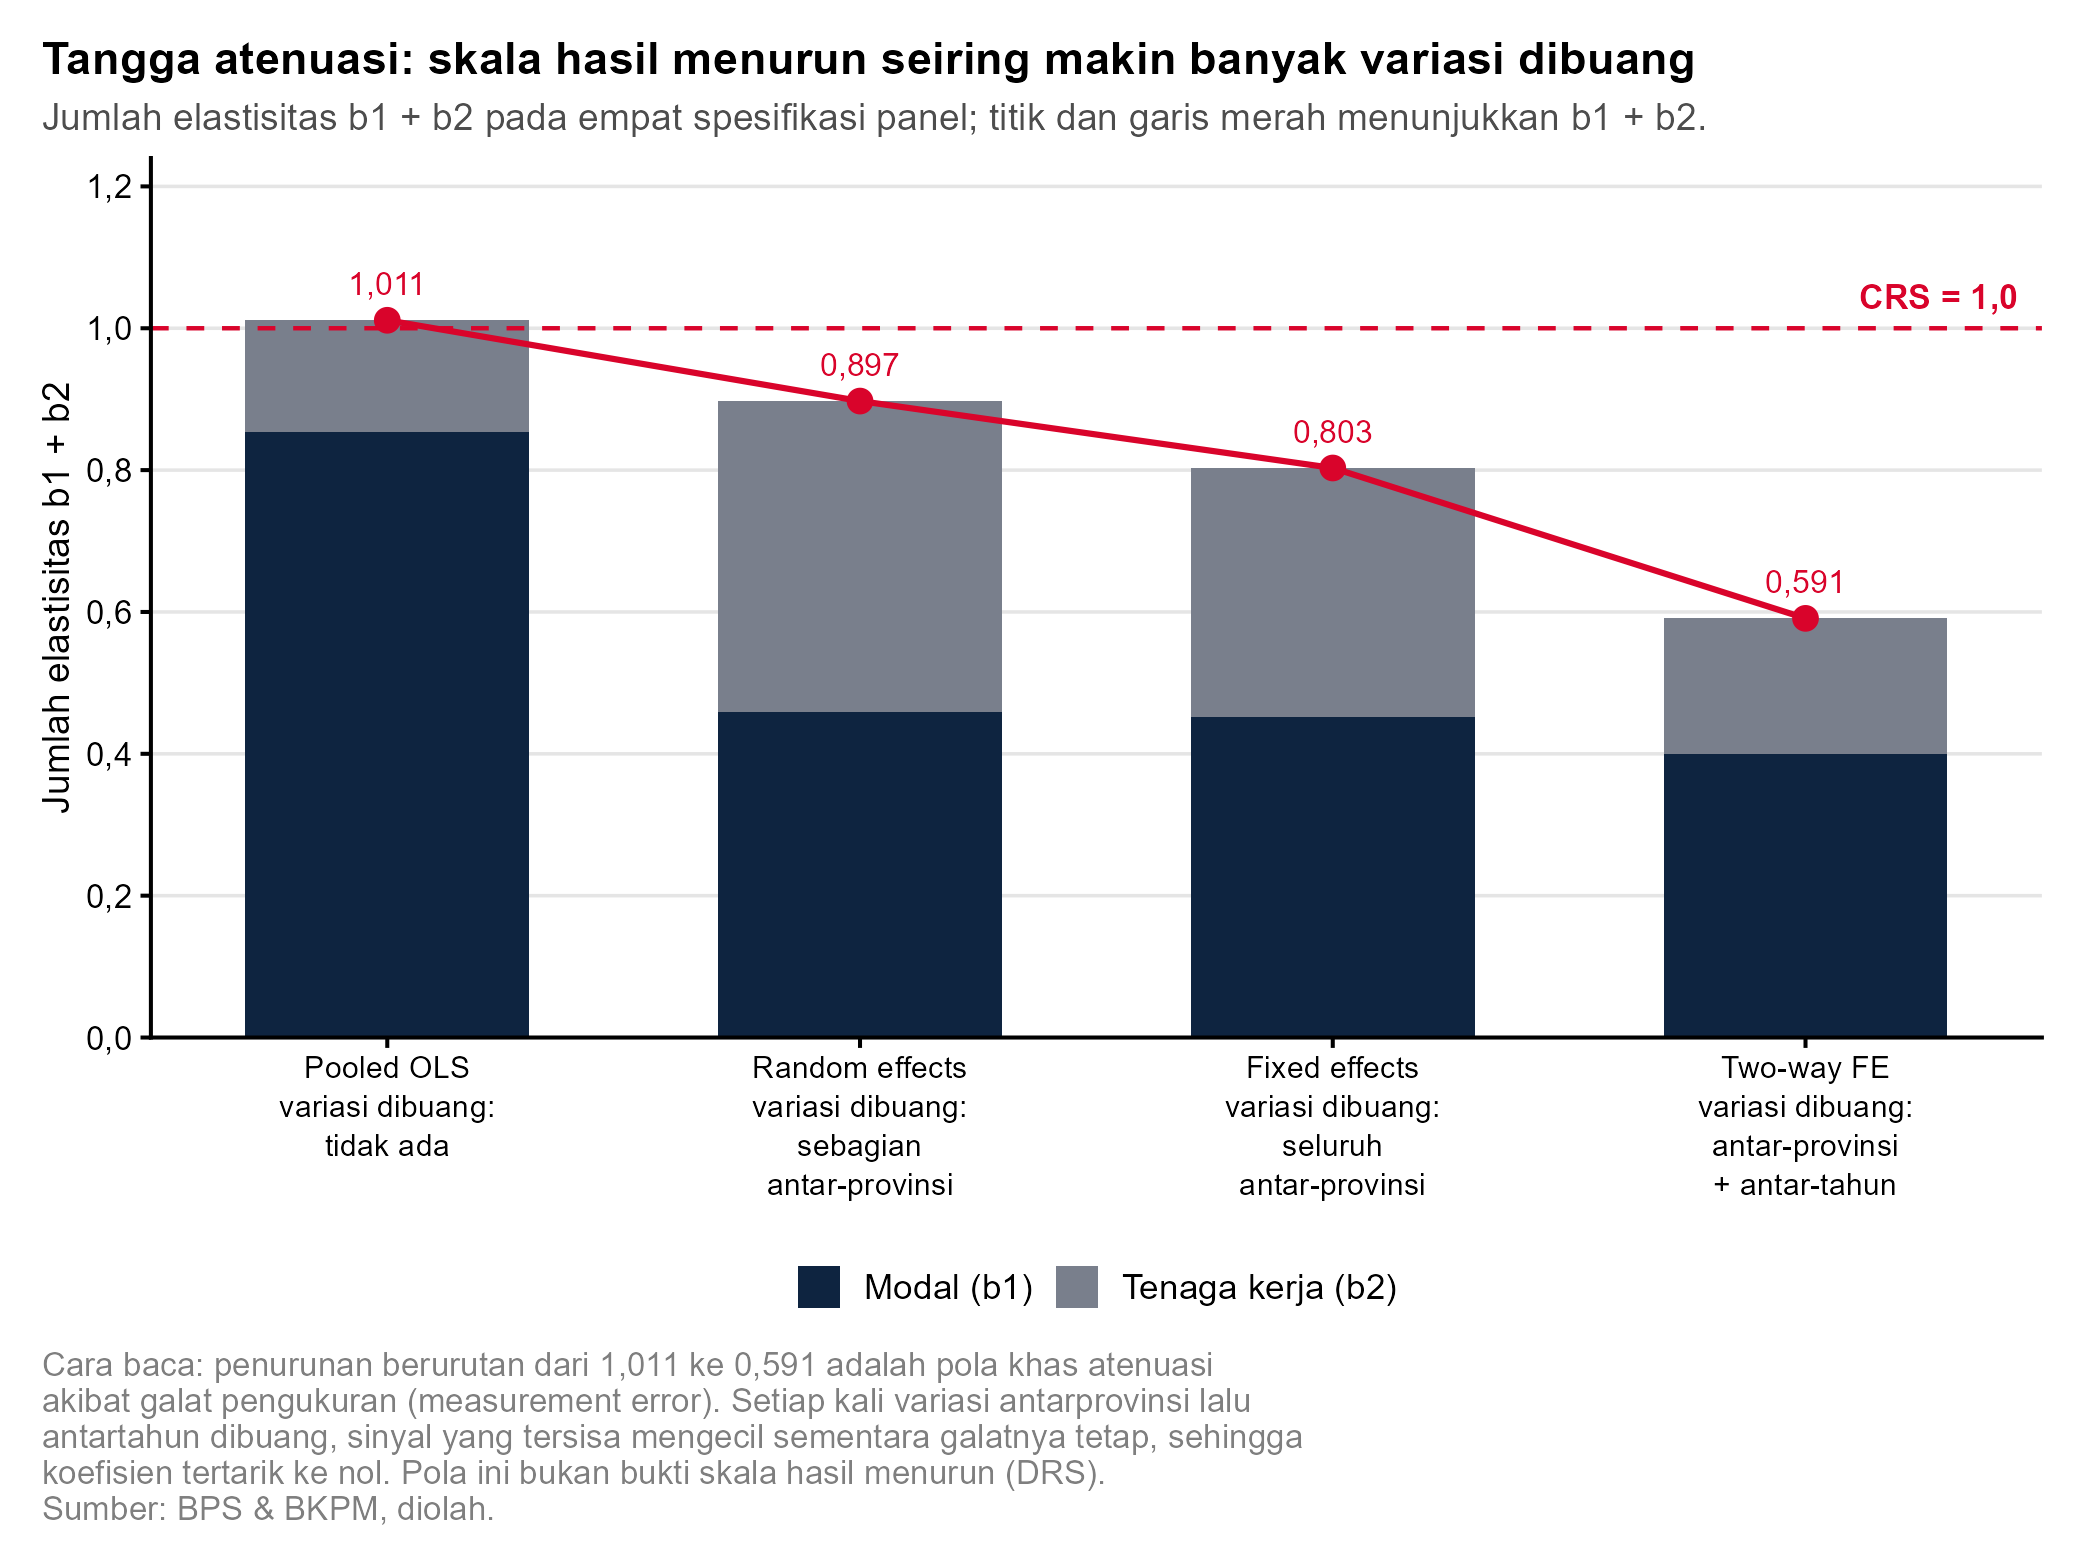
\includegraphics[width=\linewidth,keepaspectratio]{tangga_atenuasi}\\[0.3em]
      {\color{abu}\footnotesize Jumlah elastisitas turun rapi saat kontrol makin
      ketat: 1,01 (pooled) $\to$ 0,59 (dua arah).}
    \end{column}
  \end{columns}
\end{frame}

% ======================= BAGIAN 2: HASIL =======================
\begin{frame}{Angka yang berubah}
  \centering
  \renewcommand{\arraystretch}{1.35}
  \begin{tabular}{lcc}
    \toprule
    & \textbf{CRS (lama)} & \textbf{Non-CRS / DRS (baru)}\\
    \midrule
    Elastisitas modal + TK   & 0,446 + 0,554 = 1 & 0,400 + 0,191 = \key{0,591}\\
    Residual TFP             & \turun{$-$0,05 poin} & \naik{$+$0,98 poin (25,7\%)}\\
    Tren TFP nasional        & \turun{$-$0,27\%/th} & \naik{$+$0,81\%/th}\\
    Indeks TFP 2024 (2017=100)& 98,6 & \naik{106,8}\\
    Kontribusi modal         & 71\% & 64\%\\
    \bottomrule
  \end{tabular}
  \vspace{0.9em}

  {\color{abu} Modal dominan di kedua versi. Yang berubah: kesimpulan soal TFP.}
\end{frame}

\begin{frame}{TFP nasional: naik, bukan turun}
  \centering
  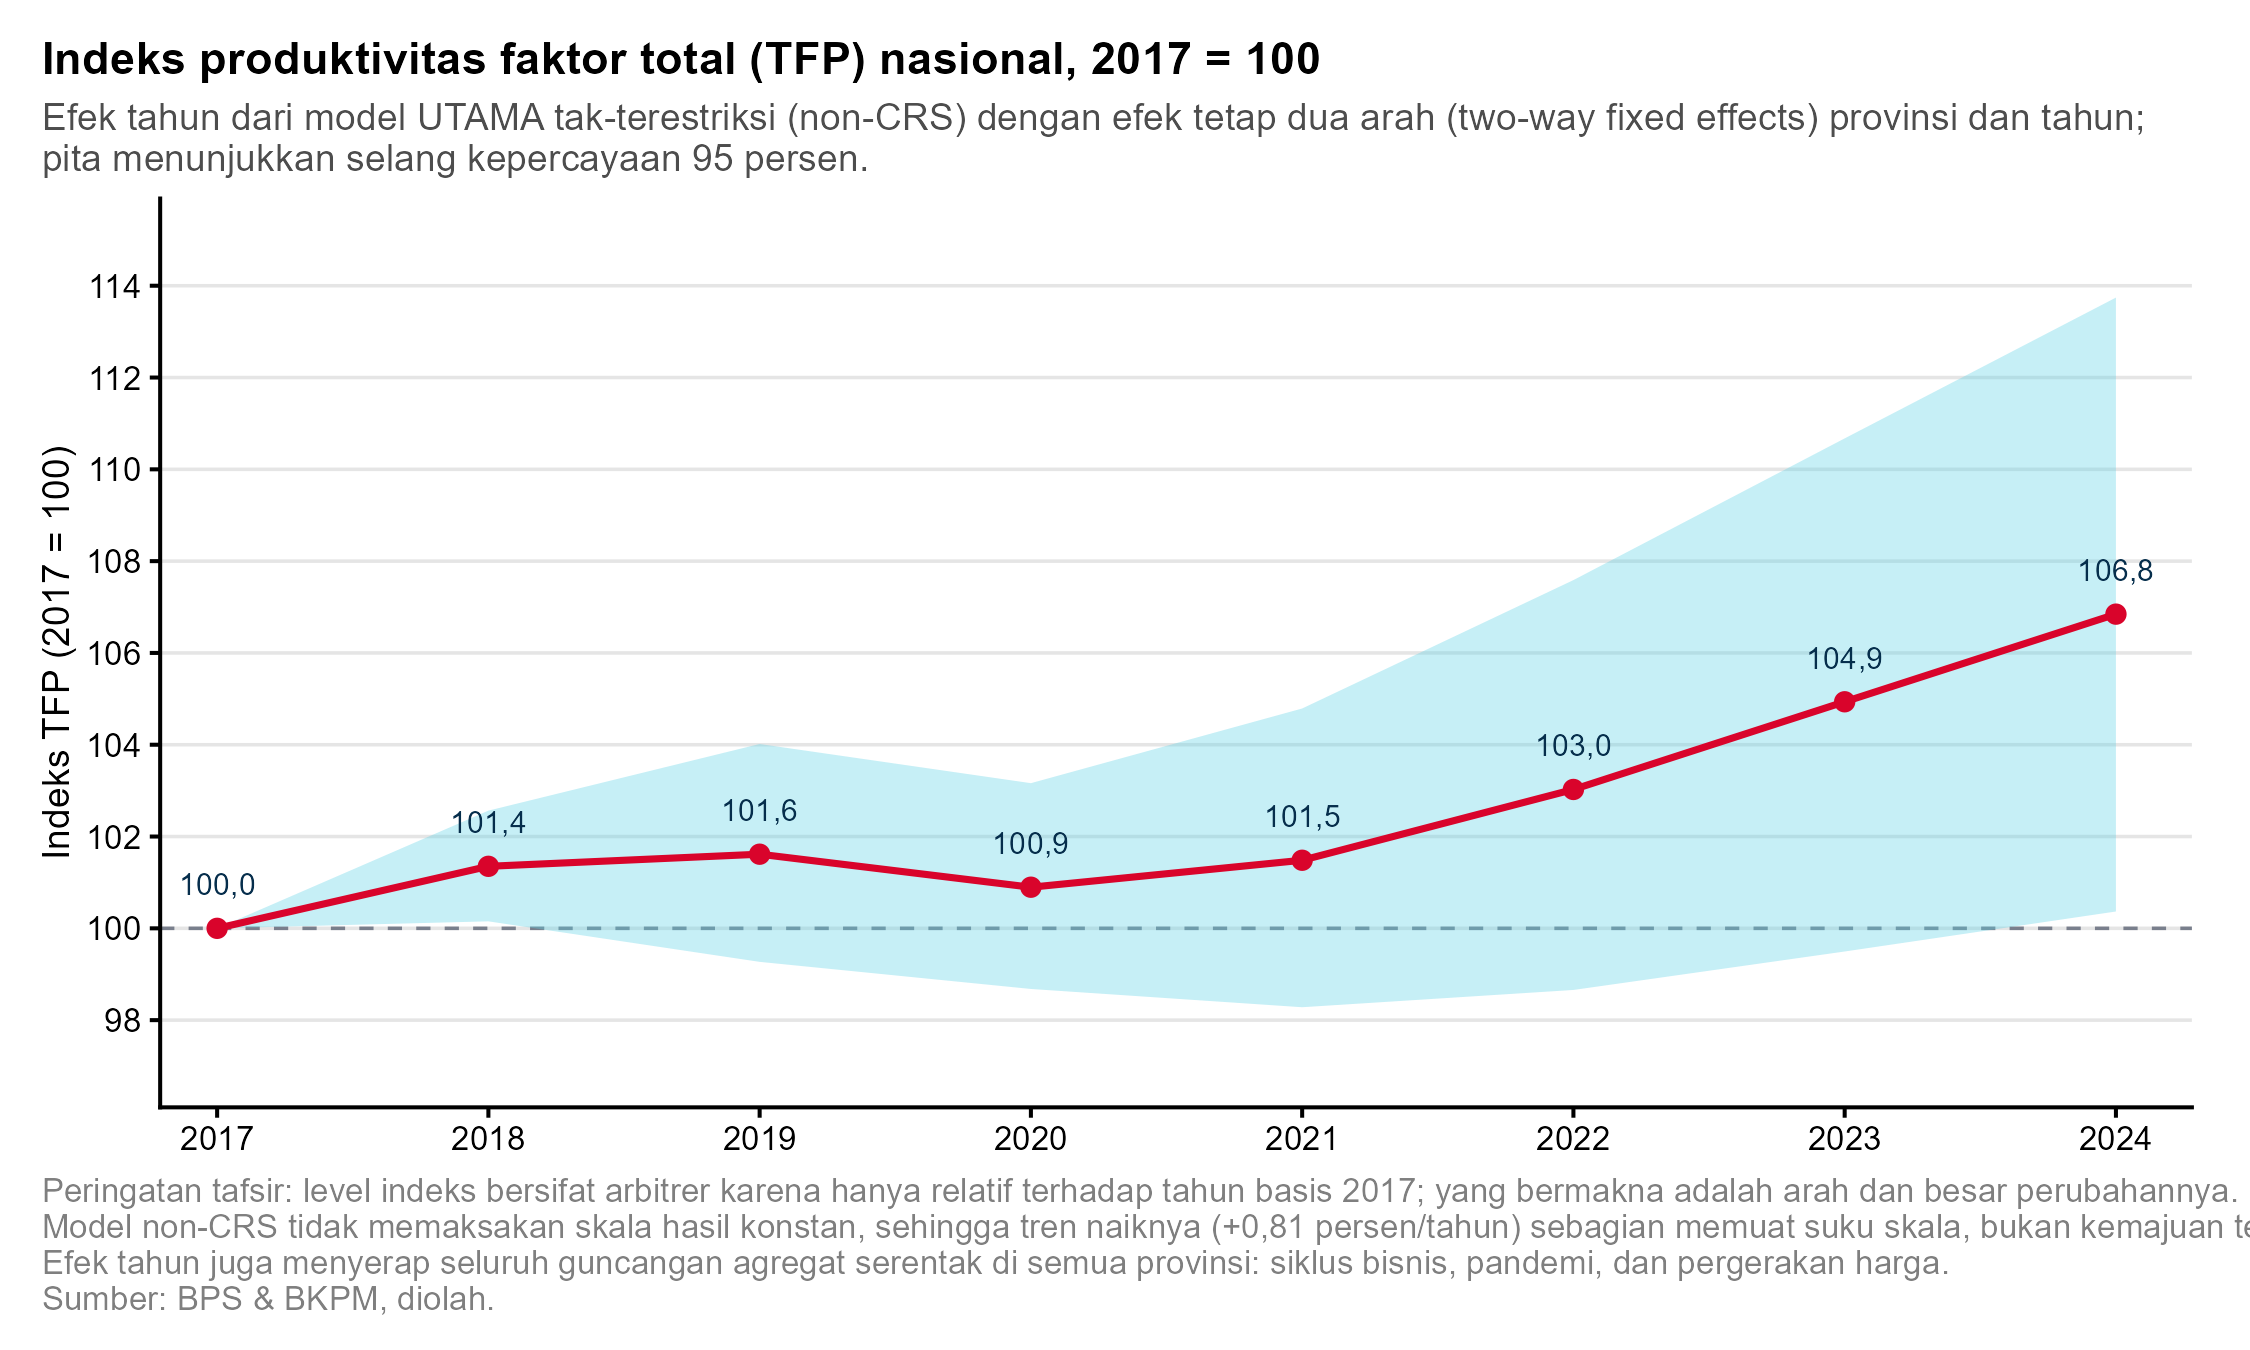
\includegraphics[height=0.70\textheight,keepaspectratio]{indeks_nasional}\\
  {\color{abu}\footnotesize Indeks dari koefisien $\lambda_t$. Cekung saat pandemi, tembus 106,8 di 2024. Tren $+0{,}81\%$/th ($p=0{,}002$).}
\end{frame}

\begin{frame}{Kontribusi tiap faktor sepanjang waktu}
  \centering
  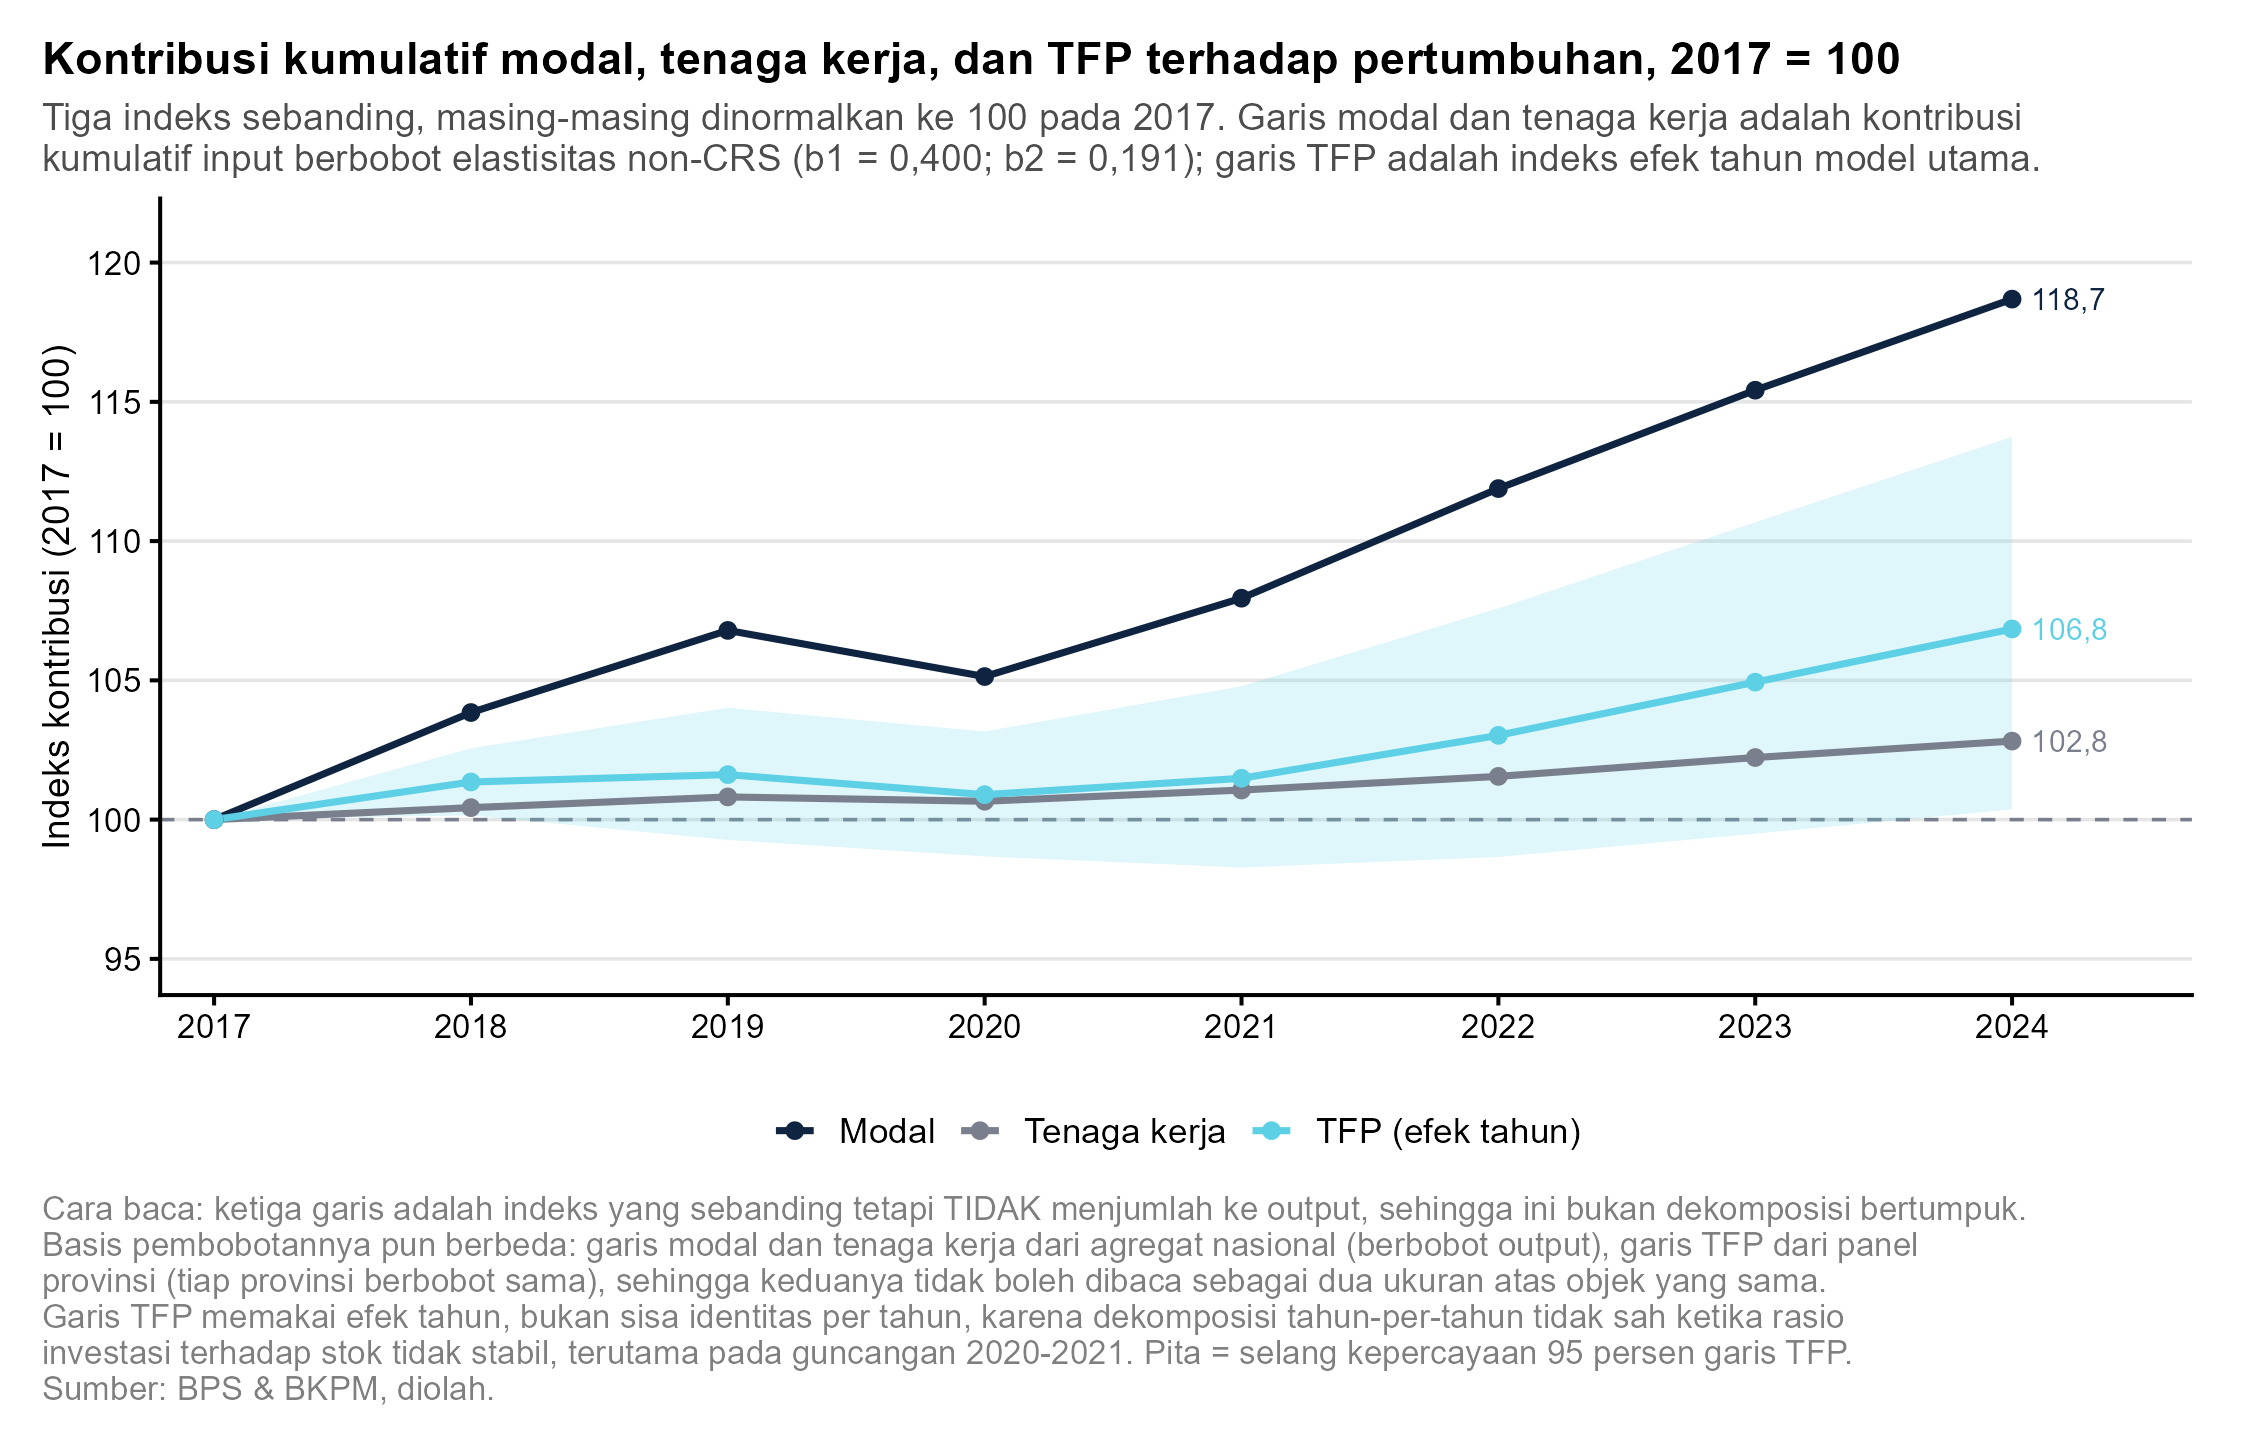
\includegraphics[height=0.68\textheight,keepaspectratio]{kontribusi_kumulatif}\\
  {\color{abu}\footnotesize Tiga indeks sebanding (2017=100), \textbf{tidak} dijumlahkan ke output.
  Modal \key{118,7} $>$ TFP \key{106,8} $>$ TK \key{102,8} di 2024; hanya modal yang berpalung saat pandemi.}
\end{frame}

\begin{frame}{Peringkat provinsi (baca hati-hati)}
  \begin{columns}[c]
    \begin{column}{0.60\textwidth}
      \centering
      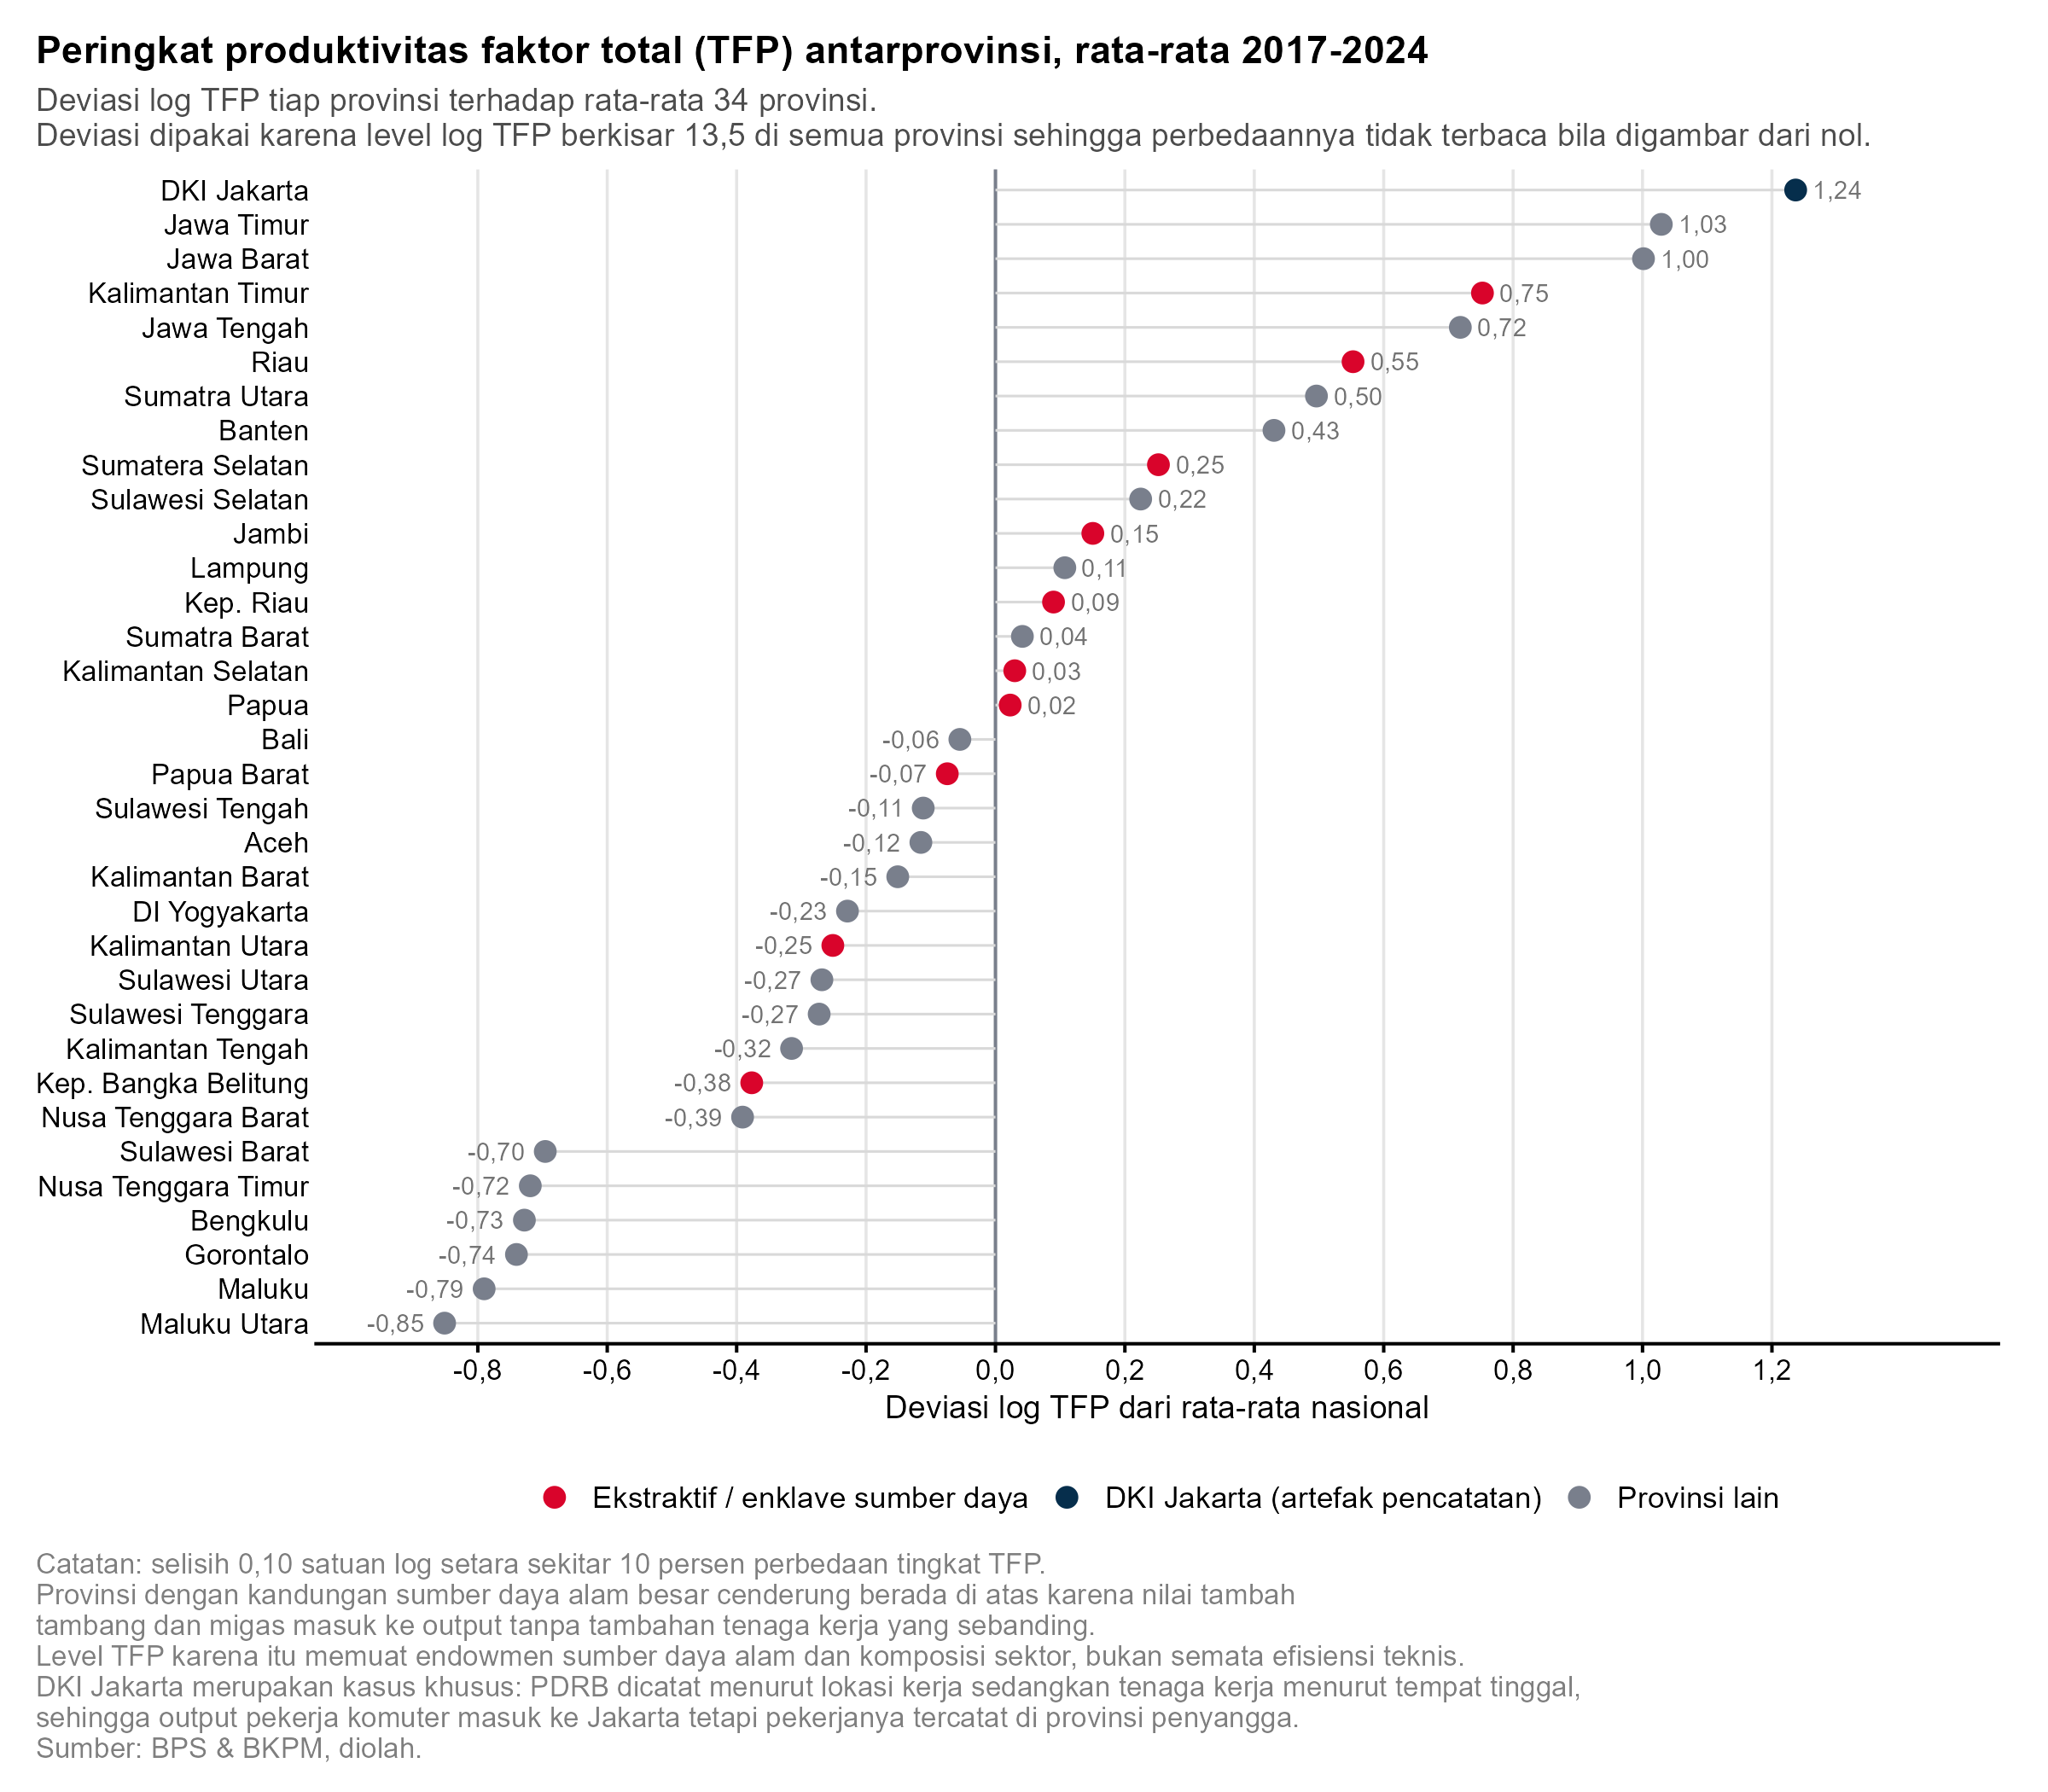
\includegraphics[width=\linewidth,keepaspectratio]{peringkat_provinsi}
    \end{column}
    \begin{column}{0.38\textwidth}
      Titik = $u_i$ tiap provinsi (deviasi dari rata-rata nasional).
      \vspace{0.7em}

      Provinsi besar (DKI, Jatim, Jabar, Kaltim) di atas.
      \vspace{0.7em}

      \key{Awas:} karena $\beta_2$ rendah (0,191), residual level ikut menyerap
      \textbf{skala tenaga kerja}. Jadi ini sebagian soal ukuran ekonomi, belum
      tentu efisiensi murni.
    \end{column}
  \end{columns}
\end{frame}

\begin{frame}{Sumber pertumbuhan: modal, jelas}
  \centering
  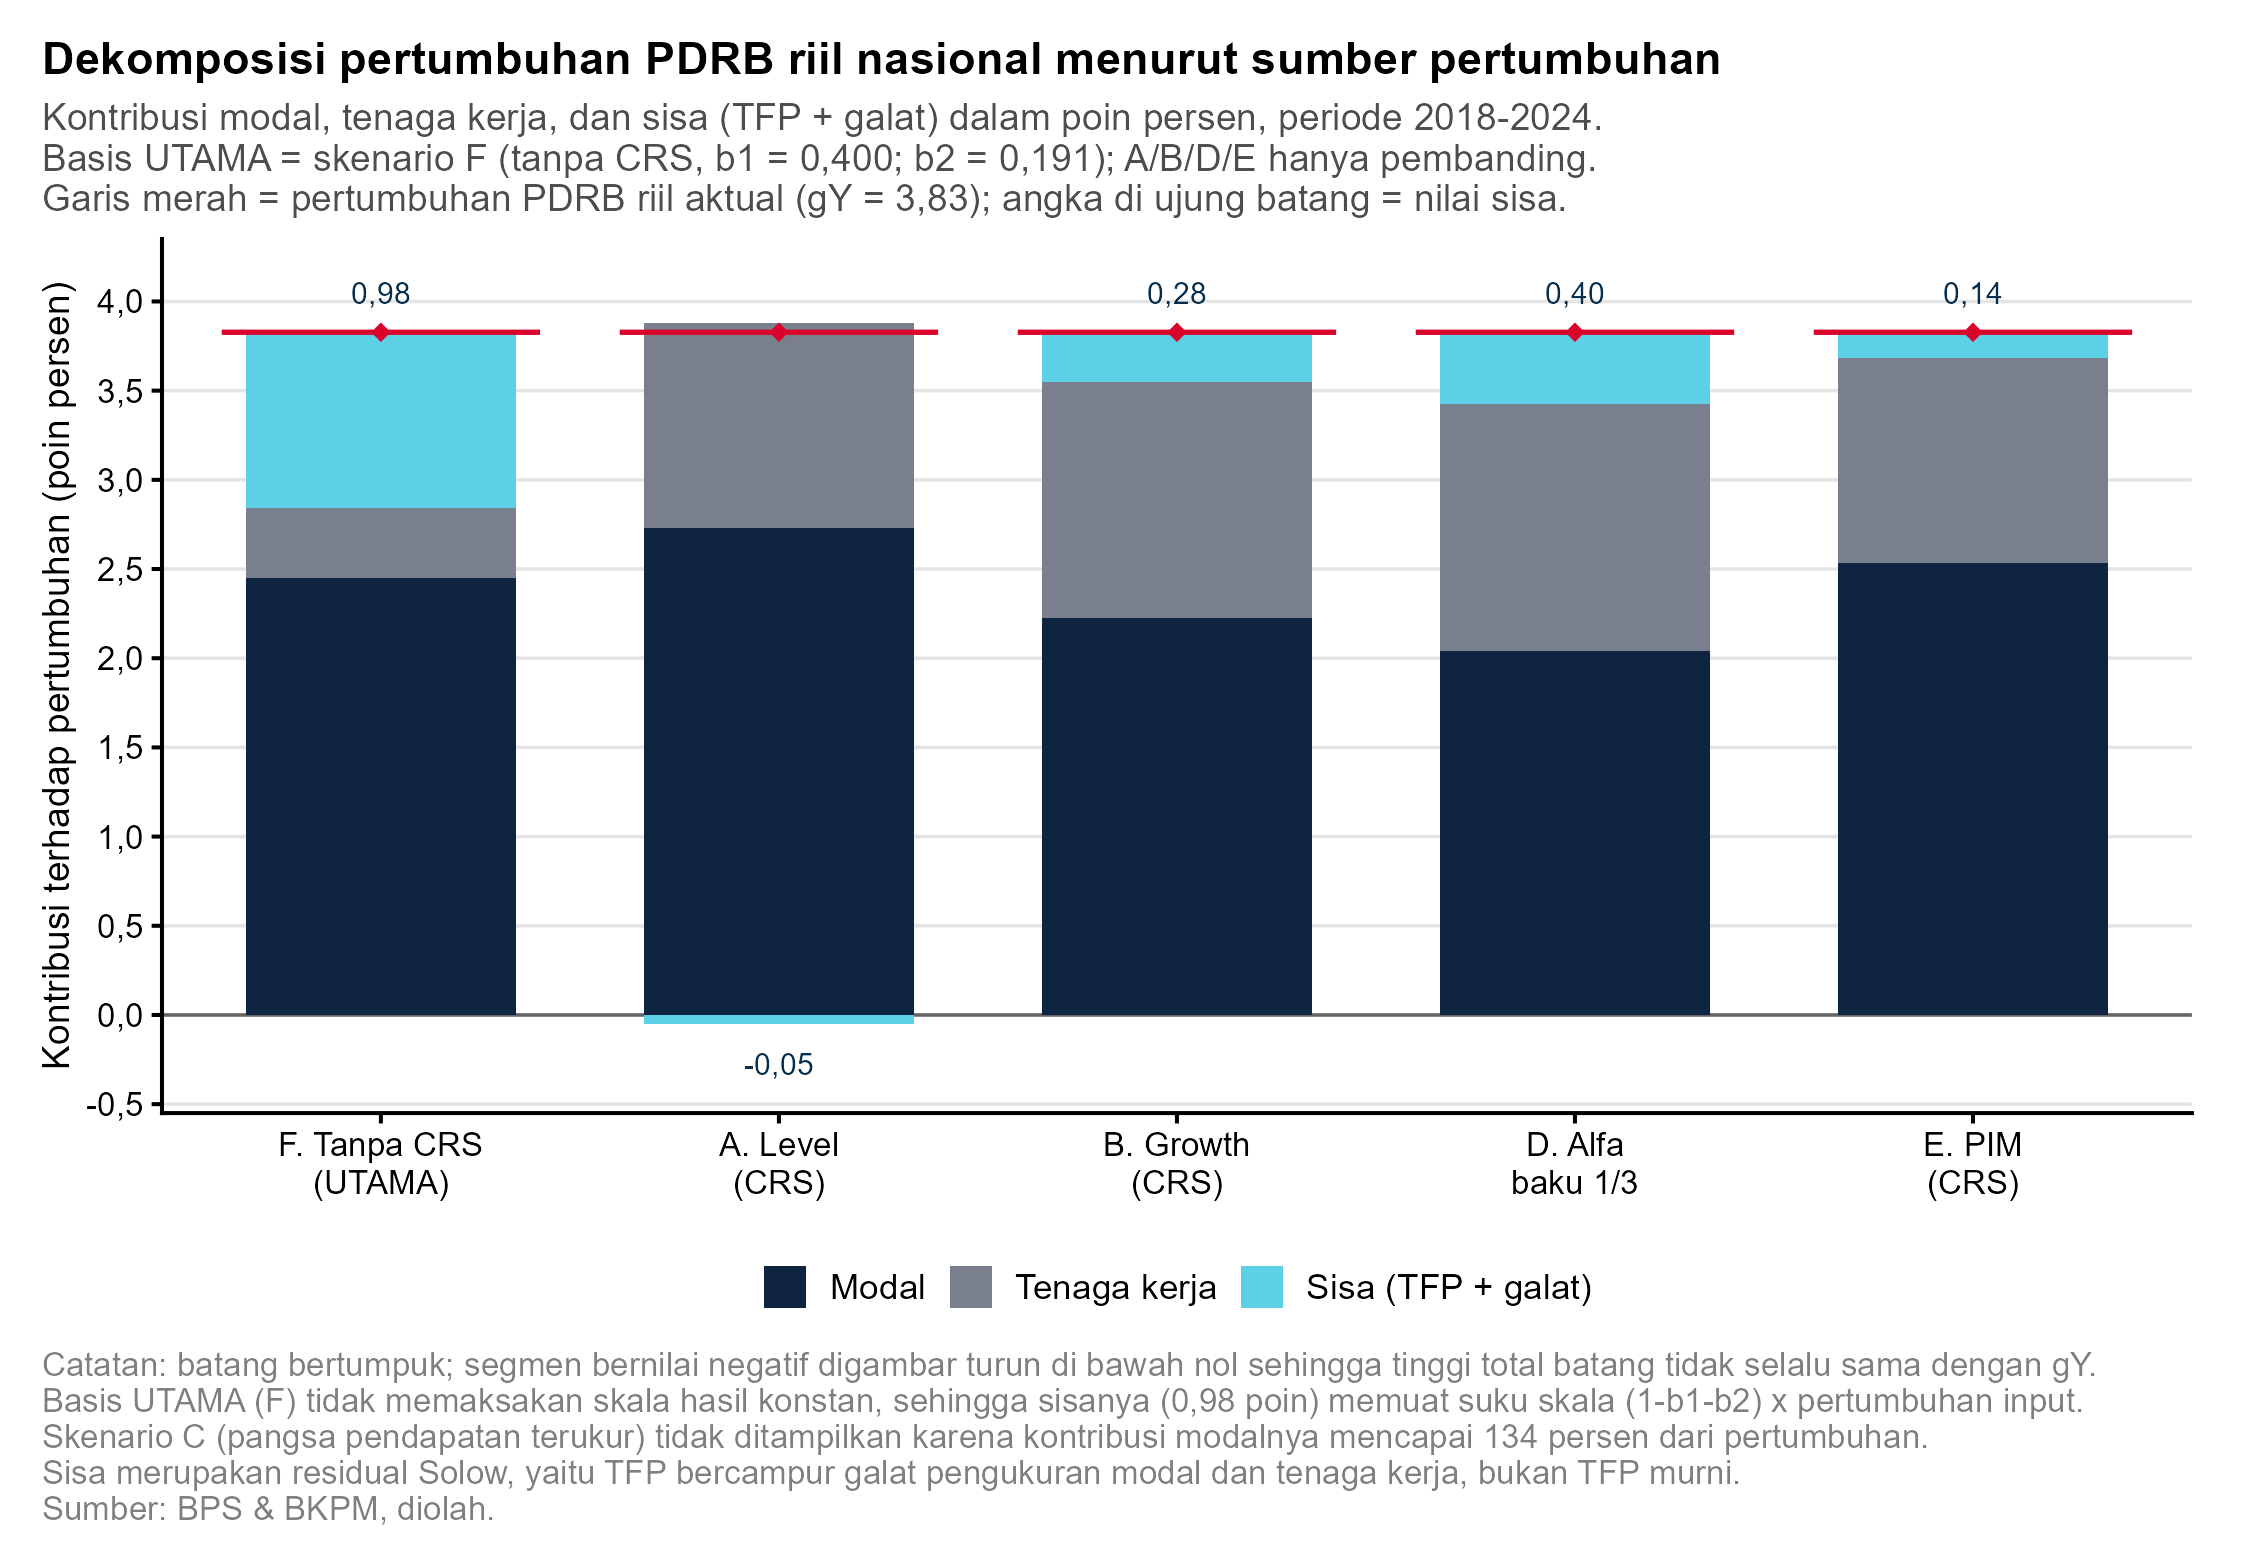
\includegraphics[height=0.70\textheight,keepaspectratio]{dekomposisi_nasional}\\
  {\color{abu}\footnotesize Batang modal jauh di atas tenaga kerja maupun sisa TFP, konsisten di semua skenario elastisitas.}
\end{frame}

\begin{frame}{Antar pulau berbeda cerita}
  \centering
  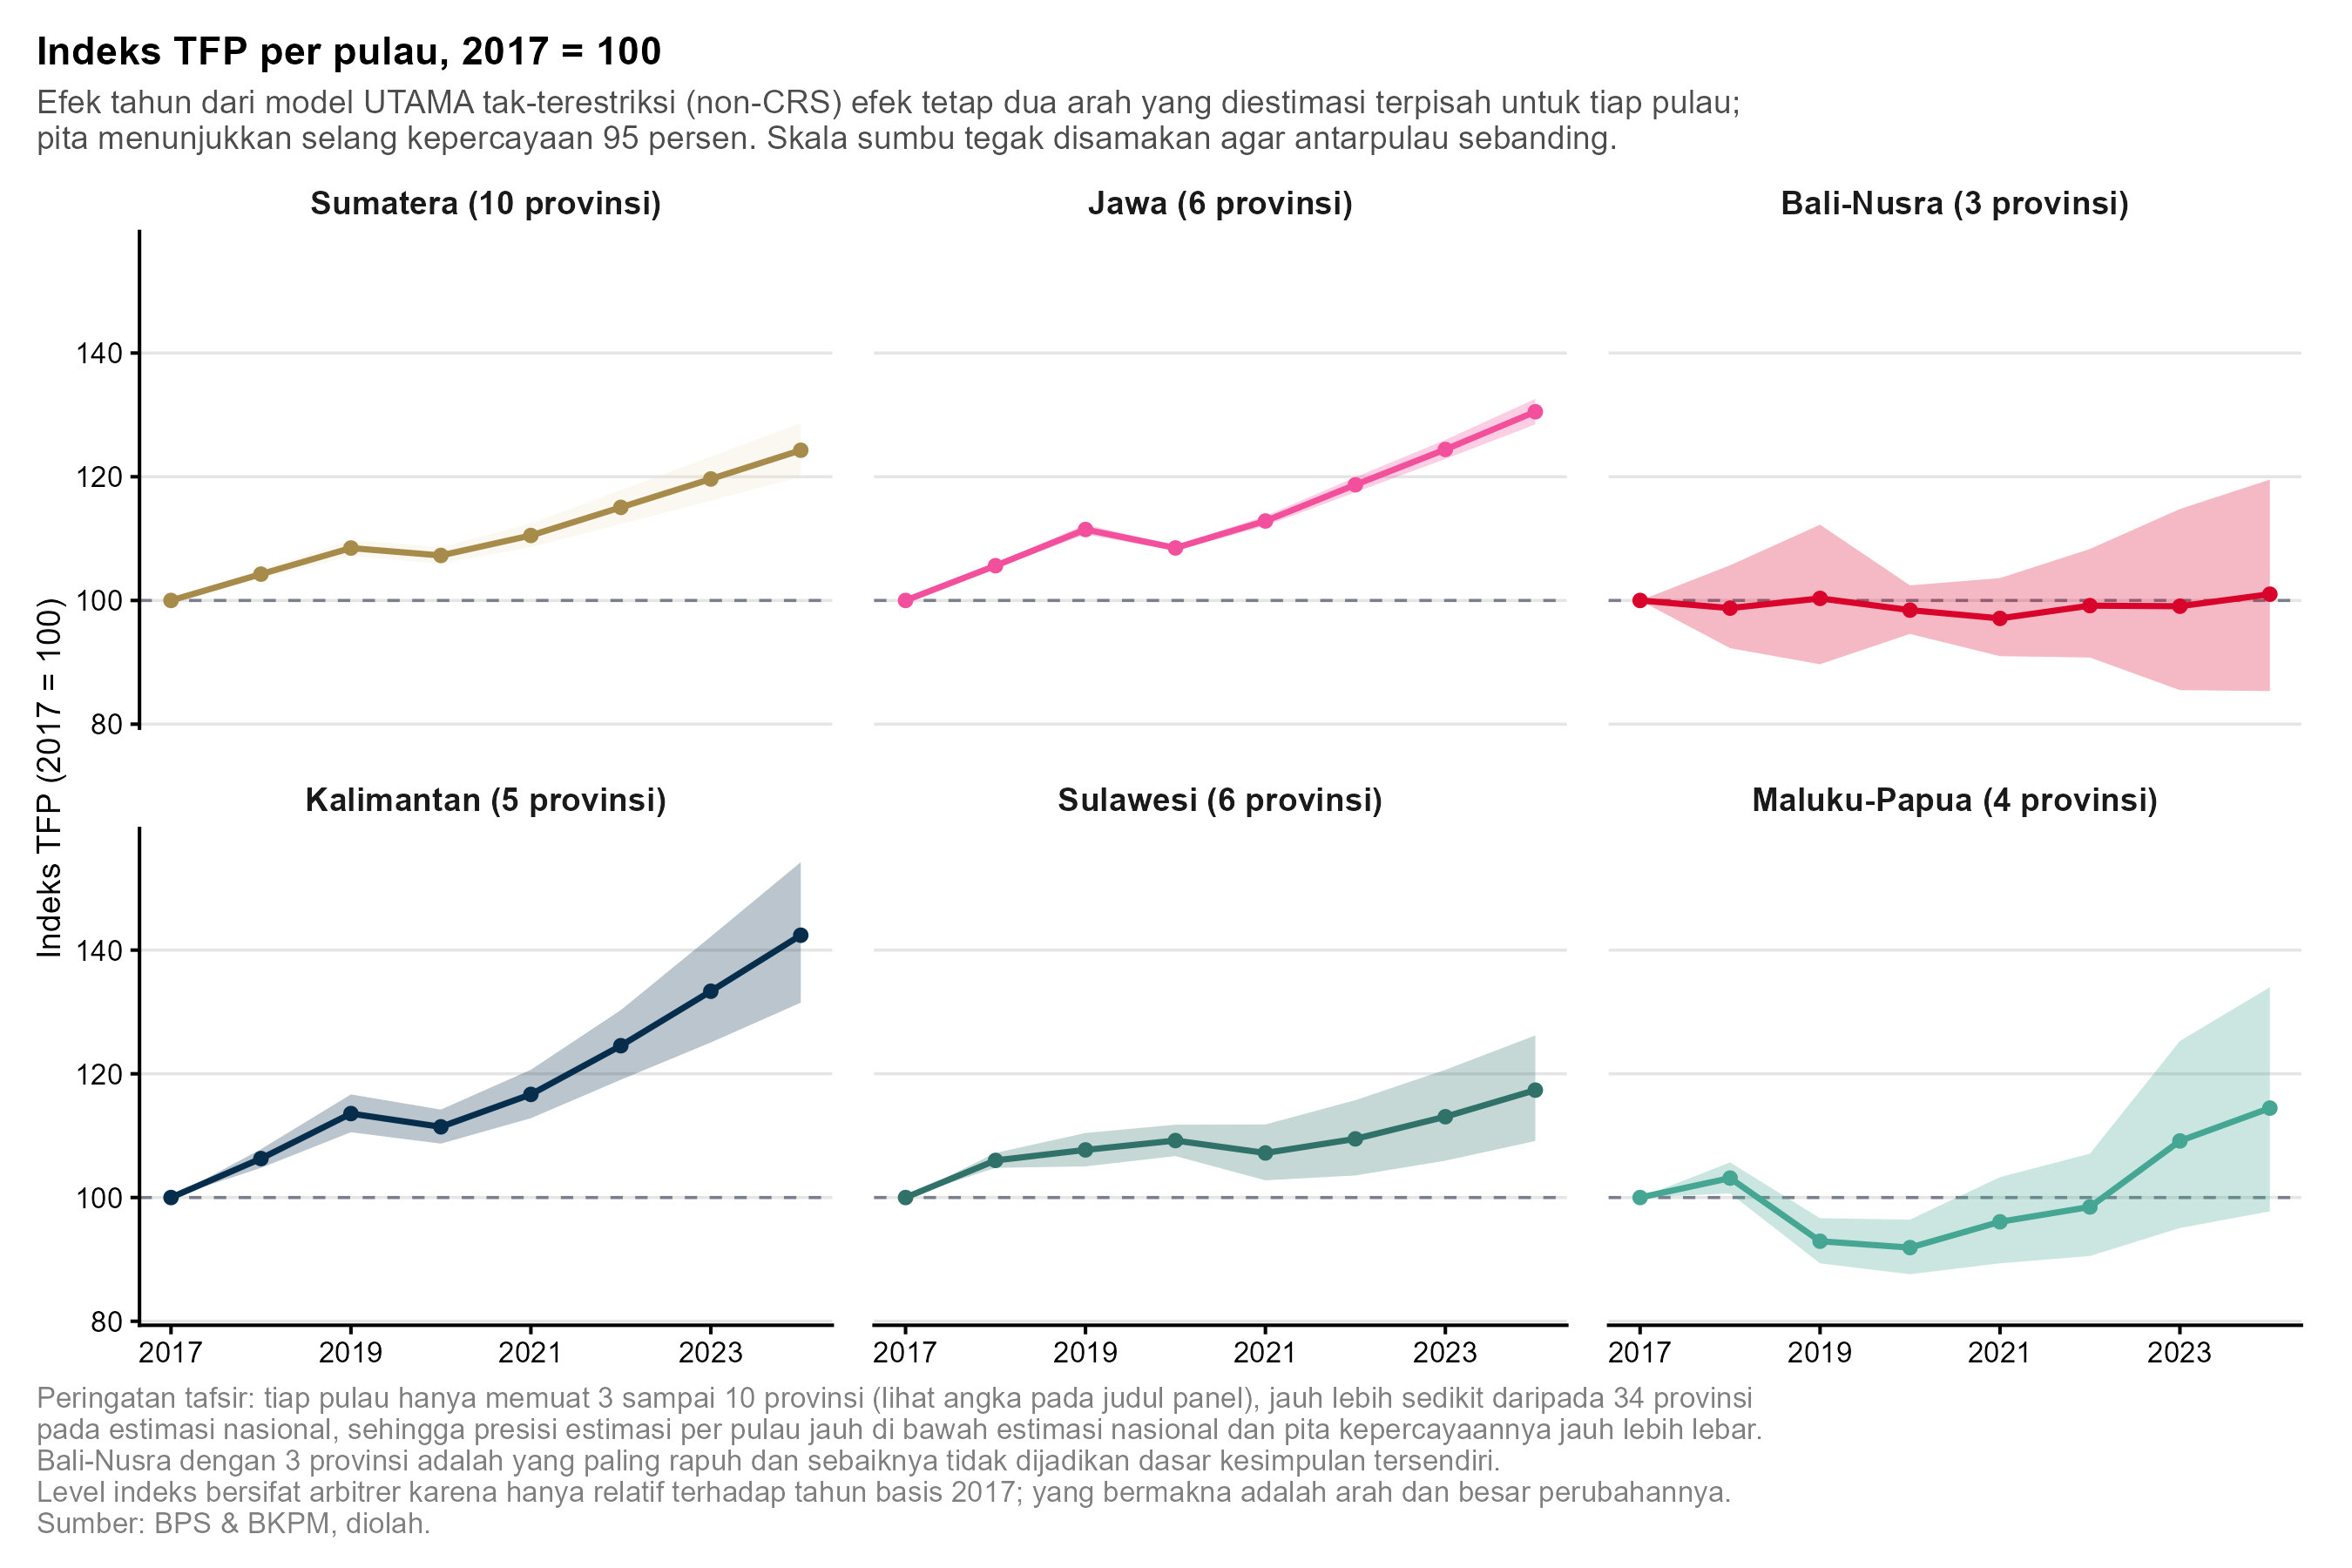
\includegraphics[height=0.70\textheight,keepaspectratio]{indeks_pulau}\\
  {\color{abu}\footnotesize Tiap pulau diestimasi terpisah. Pita lebar = presisi rendah; baca sebagai arah, bukan angka pasti.}
\end{frame}

% ======================= BAGIAN 3: SIMULASI =======================
\begin{frame}{Simulasi DRS vs CRS: apa dan kenapa}
  \textbf{Pertanyaannya:} seberapa besar sih pilihan CRS vs DRS mengubah cerita?
  \vspace{0.6em}

  Dasarnya satu \emph{growth-accounting identity}:
  \[
    g_Y = \beta_1\, g_K + \beta_2\, g_L + g_{\mathrm{TFP}}
  \]
  \begin{itemize}
    \setlength\itemsep{0.5em}
    \item Ini \emph{deterministic comparative-statics} --- \key{bukan Monte-Carlo}.
          Pertumbuhan $g_Y,g_K,g_L$ sudah tetap dari data; yang kita ubah cuma
          \textbf{asumsi $\beta$}, lalu lihat ke mana angkanya bergeser.
    \item Tiga uji: (1) \emph{reconciliation}, (2) \emph{sensitivity sweep}, (3) \emph{forward counterfactual}.
  \end{itemize}
  \vspace{0.4em}
  {\color{abu}\small Karena identitasnya eksak, tiap poin bisa diaudit sel per sel.}
\end{frame}

\begin{frame}{Blok 1 --- \emph{Reconciliation}: apa yang pindah}
  Angka pertumbuhan \textbf{sama persis} ($g_Y=3{,}83$; $g_K=6{,}12$; $g_L=2{,}08$). Hanya $\beta$ beda:
  \vspace{0.4em}
  \begin{center}
  \renewcommand{\arraystretch}{1.25}
  \begin{tabular}{lccc}
    \toprule
    & Kontribusi modal & Kontribusi TK & \textbf{Sisa (TFP)}\\
    \midrule
    \textbf{CRS} ($\beta_1{+}\beta_2{=}1$)     & 2,73 (71\%) & 1,15 & \turun{$-$0,05 ($-$1,4\%)}\\
    \textbf{DRS} ($\beta_1{+}\beta_2{=}0{,}59$) & 2,45 (64\%) & 0,40 & \naik{$+$0,98 (25,7\%)}\\
    \bottomrule
  \end{tabular}
  \end{center}
  \vspace{0.5em}
  TFP bergeser \key{1,03 poin} ($-$0,05 $\to$ $+$0,98). Tak ada yang berubah di
  ekonomi. Yang berubah cuma seberapa besar pertumbuhan kita kreditkan ke input.
  Memaksa CRS = memberi input pujian berlebih, lalu menghukum TFP.
\end{frame}

\begin{frame}{Blok 2 --- \emph{Sensitivity sweep}: tanda TFP tergantung skala}
  \begin{columns}[T]
    \begin{column}{0.52\textwidth}
      Kita geser jumlah elastisitas $\mu=\beta_1{+}\beta_2$ pelan-pelan dari
      \key{0,591} (estimasi) ke \key{1,0} (CRS), proporsi modal dijaga tetap:
      \vspace{0.5em}
      \begin{itemize}
        \setlength\itemsep{0.45em}
        \item $\mu=0{,}591 \Rightarrow$ TFP \naik{$+$0,98} (26\%)
        \item $\mu\approx0{,}80 \Rightarrow$ TFP \key{$\approx 0$} (titik nol)
        \item $\mu=1{,}0 \Rightarrow$ TFP \turun{$-$0,99} ($-$26\%)
      \end{itemize}
      \vspace{0.6em}
      \textbf{Bacaan:} TFP tetap positif selama skala di bawah $\sim$0,80.
      Estimasi kita (0,591) jelas di zona positif. TFP baru jadi negatif kalau
      kita paksa skala mendekati konstan.
    \end{column}
    \begin{column}{0.46\textwidth}
      \centering
      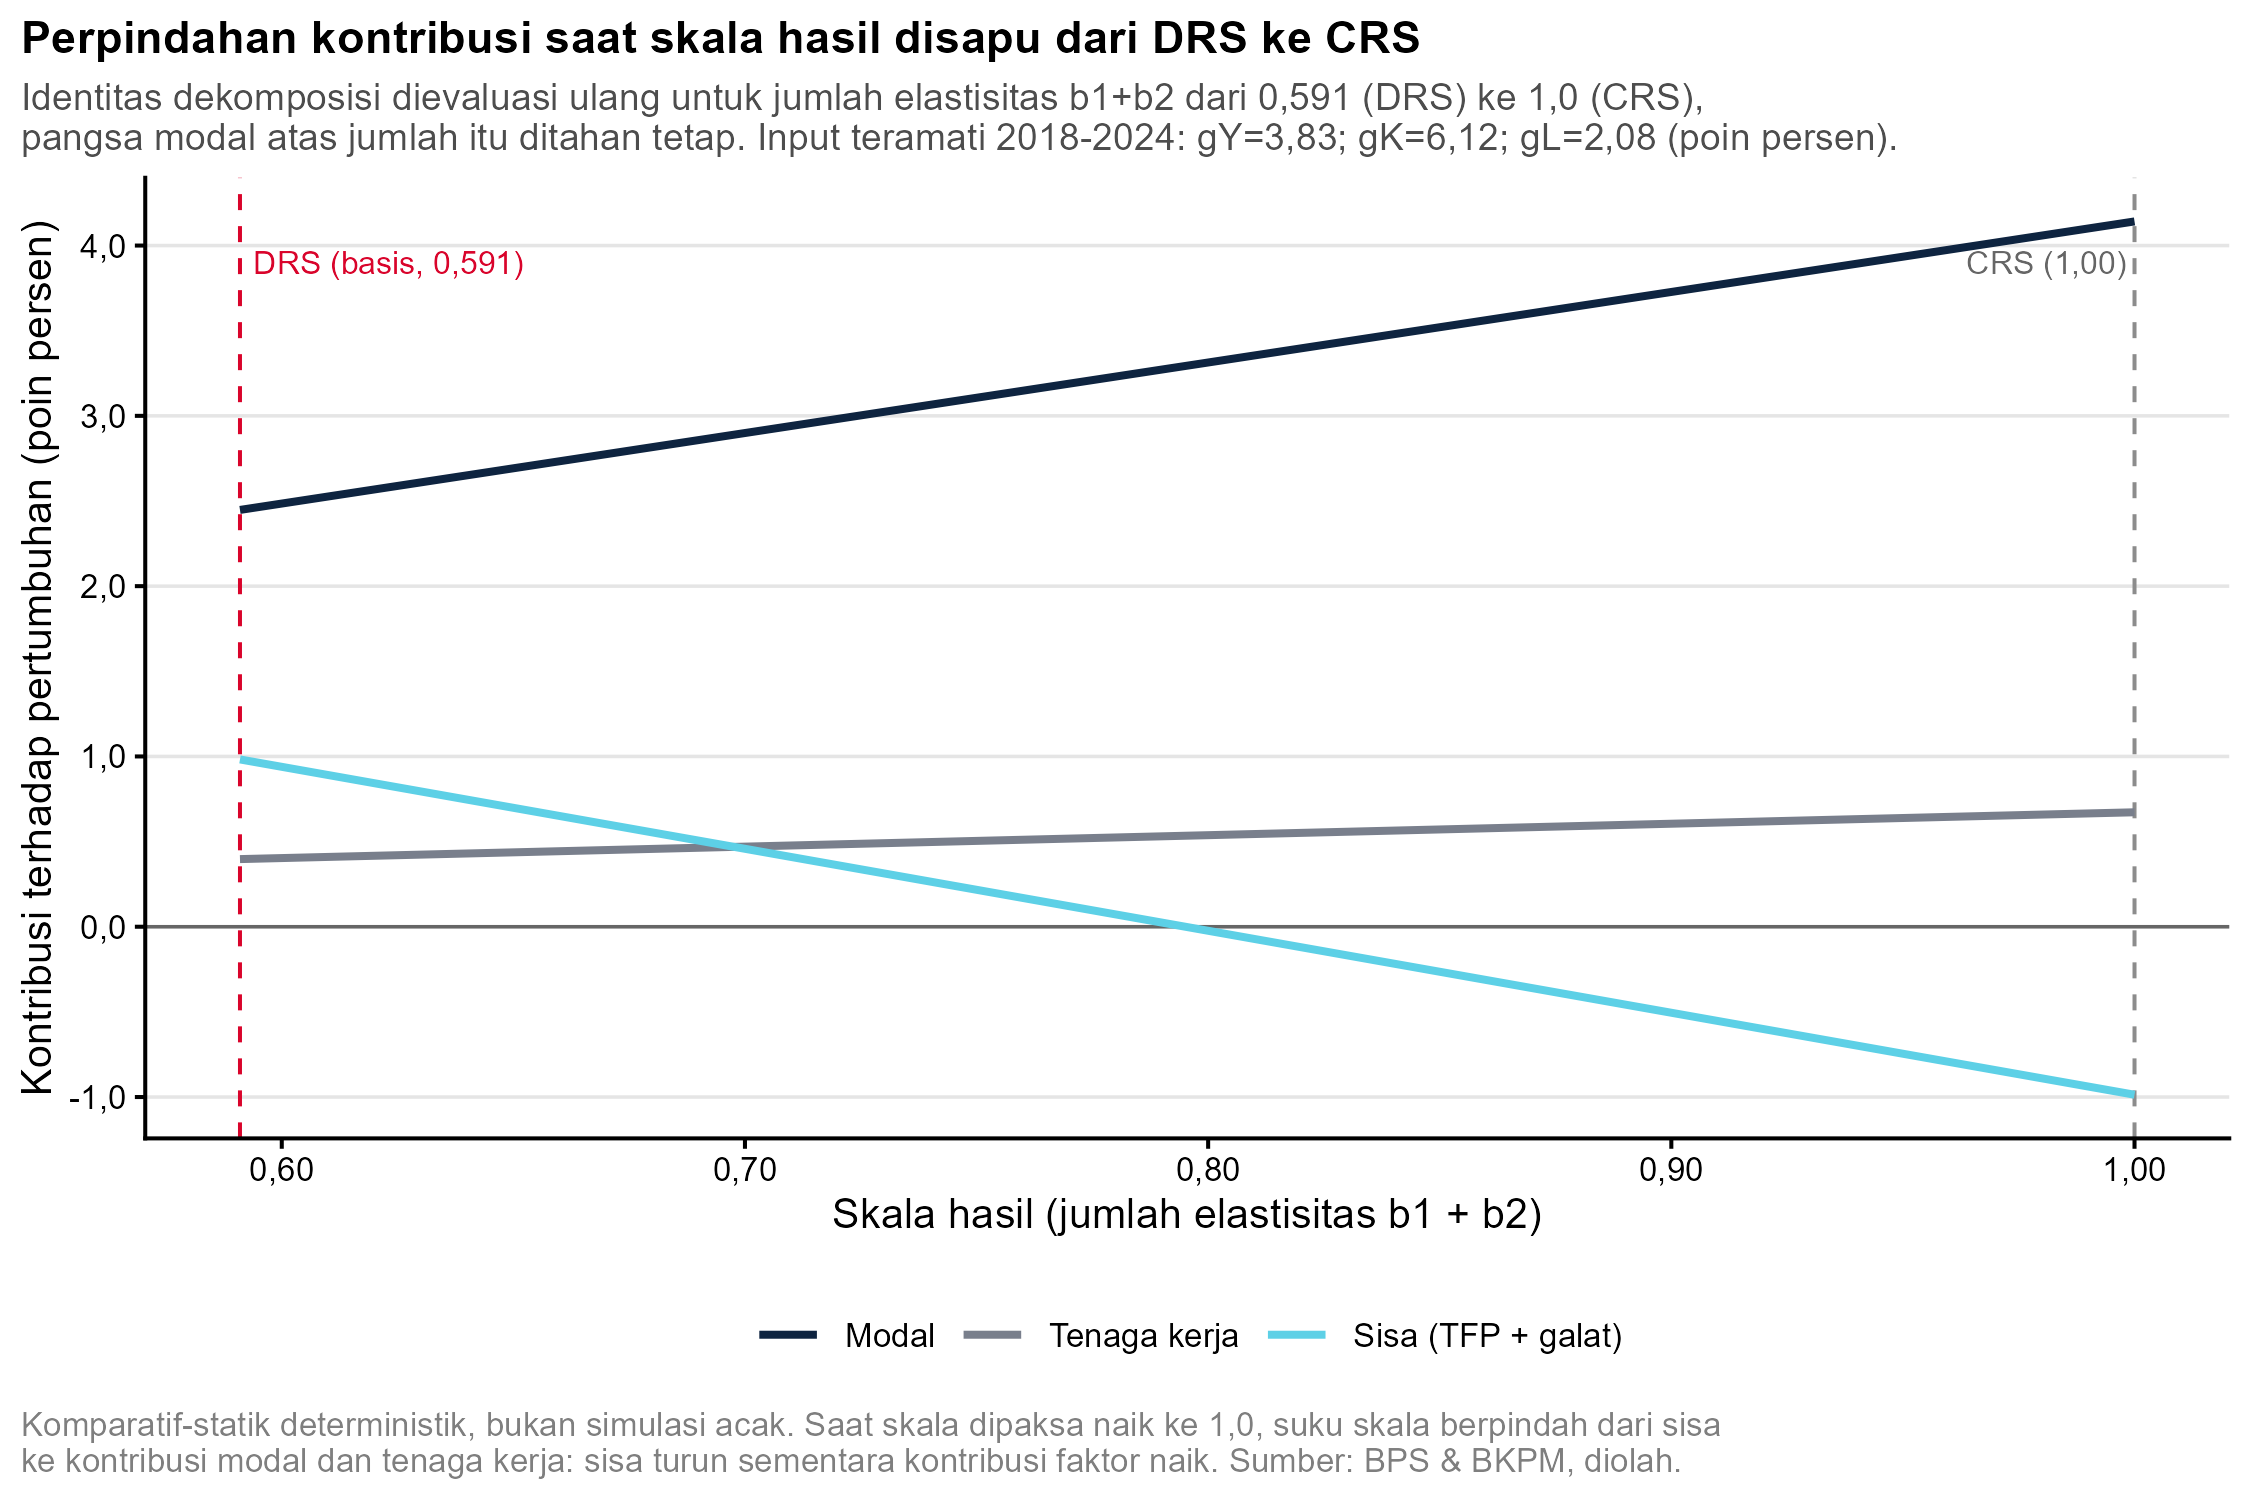
\includegraphics[width=\linewidth,keepaspectratio]{simulasi}\\
      {\color{abu}\footnotesize Tiga panel: \emph{reconciliation}, \emph{sensitivity sweep}, \emph{counterfactual}.}
    \end{column}
  \end{columns}
\end{frame}

\begin{frame}{Blok 3 --- \emph{Counterfactual}: berapa TFP yang dibutuhkan?}
  Balik pertanyaannya: untuk mengejar \key{output 8\%/th}, berapa TFP yang harus
  tumbuh, mengingat input hanya mengangkat sebagian?
  \vspace{0.3em}
  \begin{center}
  \renewcommand{\arraystretch}{1.25}
  \begin{tabular}{lcc}
    \toprule
    & \textbf{TFP dibutuhkan (CRS)} & \textbf{TFP dibutuhkan (DRS)}\\
    \midrule
    Modal teramati ($g_K=6{,}1$)      & 4,12\%/th & \key{5,16\%/th}\\
    Modal cepat ($g_K=12$, 8-4-2-2)   & 1,50\%/th & \key{2,81\%/th}\\
    \bottomrule
  \end{tabular}
  \end{center}
  \vspace{0.5em}
  \begin{itemize}
    \setlength\itemsep{0.4em}
    \item DRS menuntut TFP \key{lebih tinggi} karena input dikreditkan lebih hemat.
    \item Bandingkan dengan realita: TFP cuma tumbuh $\sim$0,81\%/th.
    \item Artinya \key{target 8\% sangat berat} begitu kita berhenti mengover-kredit input --- bahkan dengan investasi digenjot ke 12\%.
  \end{itemize}
\end{frame}

% ======================= BAGIAN 4: BATAS & PESAN =======================
\begin{frame}{Jujur soal batasnya}
  \begin{itemize}
    \setlength\itemsep{0.8em}
    \item Modal kita proksi dari \key{PMTB (aliran)}, bukan stok kapital. Proksi
          aliran + \emph{within transformation} menekan $\beta_1$ ke bawah (\emph{attenuation bias}).
    \item Maka \textbf{sebagian} penolakan CRS bisa efek pengukuran, bukan DRS
          sejati (Griliches--Mairesse 1998; Basu--Fernald 1997).
    \item Baca TFP \naik{$+$0,98 poin} sebagai \key{batas atas}. Kontribusi TFP
          sesungguhnya ada di antara $\sim$0 dan 0,98 --- condong ke bawah.
  \end{itemize}
  \vfill
  {\color{abu}\small Justru caveat ini yang membuat angkanya bertahan di depan penguji.}
\end{frame}

\begin{frame}{Ringkasan analisis}
  \large
  \begin{enumerate}
    \setlength\itemsep{0.8em}
    \item \key{Modal penggerak utama}: 64\% pertumbuhan pada basis non-CRS, konsisten di semua skenario elastisitas.
    \item \key{TFP positif tapi tipis}: $\sim$0,8\%/th, dan sebagian menyerap pemulihan utilisasi pasca-pandemi.
    \item \key{Angka provinsi/pulau rapuh}: presisi rendah dan sensitif asumsi --- baca sebagai arah, bukan angka pasti.
  \end{enumerate}
\end{frame}

\begin{frame}[plain]
  \centering\vfill
  {\color{aksen}\Huge \textbf{Terima kasih}}\\[1em]
  {\color{abu}\large Metode \& angka lengkap: \texttt{Report TFP\_0721}}
  \vfill
\end{frame}

\end{document}
